\documentclass[12pt]{amsart}
\usepackage{latexsym}
\usepackage{amssymb,amsmath}
\usepackage[pdftex]{graphicx}
\usepackage{enumerate}
\usepackage{endnotes}
%\usepackage{extpfeil}
\usepackage{hyperref}
\usepackage[usenames,dvipsnames]{xcolor}
\usepackage{stackrel}
\usepackage{bbm}
\usepackage{tikz}
\usepackage[margin=1.25in]{geometry}
\usepackage{hyperref}
\usepackage{listings}
\usepackage{courier}
\usepackage{color}
\usepackage{upgreek}

\lstset{
	basicstyle=\small\ttfamily,
	keywordstyle=\color{blue},
	language=python,
	xleftmargin=16pt,
}

\usetikzlibrary{arrows,chains,matrix,positioning,scopes}

\makeatletter
\tikzset{join/.code=\tikzset{after node path={%
\ifx\tikzchainprevious\pgfutil@empty\else(\tikzchainprevious)%
edge[every join]#1(\tikzchaincurrent)\fi}}}
\makeatother
%
\tikzset{>=stealth',every on chain/.append style={join},
         every join/.style={->}}
\tikzstyle{labeled}=[execute at begin node=$\scriptstyle,
   execute at end node=$]
\usetikzlibrary{patterns}

\usetikzlibrary{decorations.pathreplacing}

\DeclareSymbolFont{bbold}{U}{bbold}{m}{n}
\DeclareSymbolFontAlphabet{\mathbbold}{bbold}

\newtheorem{thm}{Theorem}[section]
\newtheorem{ithm}{Theorem}
\newtheorem{lem}[thm]{Lemma}
\newtheorem{conj}[thm]{Conjecture}
\newtheorem{prop}[thm]{Proposition}
\newtheorem{cor}[thm]{Corollary}

\theoremstyle{definition}
\newtheorem{defi}[thm]{Definition}
\newtheorem{example}[thm]{Example}
\newtheorem{exercise}[thm]{Exercise}
\newtheorem{rem}[thm]{Remark}


   
\def\B{{\mathbb B}}
\def\C{{\mathbb C}}
\def\D{{\mathbb D}}
\def\Fp{{\mathbb F}_p}
\def\Fell{{\mathbb F}_{\ell}}
\def\F{{\mathbb F}}
%\def\H{{\mathbb H}}
\def\M{{\mathbb M}}
\def\N{{\mathbb N}}
\def\O{{\mathcal O}}
\def\0{{\mathbb 0}}
\def\P{{{\mathbb P}}}
\def\Q{{\mathbb Q}}
\def\R{{\mathbb R}}
\def\T{{\mathbb T}}
\def\Z{{\mathbb Z}}

\newcommand{\sol}{_{a^p,b^p,c^p}}
\newcommand{\bound}{\partial}
\newcommand{\la}[1]{\mathfrak{#1}}
\newcommand{\im}{\text{Im} \hspace{0.1em} }
\newcommand{\ann}{\text{Ann} \hspace{0.1em} }
\newcommand{\rank}{\text{rank} \hspace{0.1em} }
\newcommand{\coker}[1]{\text{coker}\hspace{0.1em}{#1}}
\newcommand{\sgn}{\text{sgn}}
\newcommand{\lcm}{\text{lcm}}
\newcommand{\re}{\text{Re}  \hspace{0.1em} }
\newcommand{\ext}[1]{\text{Ext}(#1)}
\newcommand{\Hom}[1]{\text{Hom}(#1)}
\newcommand{\End}[1]{\text{End(#1)}}
\newcommand{\bs}{\setminus}
\newcommand{\rpp}[1]{\mathbb{R}\text{P}^{#1}}
\newcommand{\cpp}[1]{\mathbb{C}\text{P}^{#1}}
\newcommand{\tr}{\text{tr}\hspace{0.1em} }
\newcommand{\inner}[1]{\langle {#1}\rangle}
\newcommand{\tensor}{\otimes}
\newcommand{\Cl}{\text{Cl}}
\renewcommand{\sp}[1]{\text{Sp}_{#1}}
\newcommand{\GL}{\text{GL}}
\newcommand{\PGL}{\text{PGL}}
\renewcommand{\sl}[1]{\text{SL}_{#1}}
\newcommand{\so}[1]{\text{SO}_{#1}}
\newcommand{\SO}{\text{SO}}
\newcommand{\pso}[1]{\text{PSO}_{#1}}
\renewcommand{\o}[1]{\text{O}_{#1}}
\renewcommand{\sp}[1]{\text{Sp}_{#1}}
\newcommand{\psp}[1]{\text{PSp}_{#1}}
\newcommand{\Span}{\rm Span}
\newcommand{\Frob}{\rm Frob}
\newcommand{\tor}{\rm tor}
\newcommand{\rad}{\rm rad}
\newcommand{\denom}{\rm denom}
\renewcommand{\bar}{\overline}
\newcommand{\notdiv}{\nmid}
\newcommand{\pfrac}[2]{\left( \frac{#1}{#2} \right)}
\newcommand{\bfrac}[2]{\left| \frac{#1}{#2} \right|}
\newcommand{\Ell}{\rm Ell}
\newcommand{\AV}{\rm AV}
\newcommand{\Gal}{\rm Gal}

\newcommand{\kron}[2]{\bigl(\frac{#1}{#2}\bigr)}
\newcommand{\leg}[2]{\Biggl(\frac{#1}{#2}\Biggr)}

\DeclareSymbolFont{bbold}{U}{bbold}{m}{n}
\DeclareSymbolFontAlphabet{\mathbbold}{bbold}

\begin{document}

\title{Perfect Powers in Lucas Sequences via Galois Representations}
\author{Jesse Silliman and Isabel Vogt}

\maketitle


\section{Introduction and Statement of Results}
The Fibonacci Sequence, perhaps the simplest linear recurrence relation, begins as \[0,\underline{1},\underline{1},2,3,5,\underline{8},13,21,34,55,89,\underline{144},233.\] Note that the underlined terms are perfect powers. It was a folklore conjecture that these terms are in fact the only perfect powers in the Fibonacci sequence. Various partial results in this direction, using classical methods, ruled out other $p$-th powers for small primes $p$. Finally, in a deep paper \cite{siksek06}, the conjecture was proven. However, in contrast with previous results, this proof relied upon the Modularity Theorem of Wiles et al., connecting the Diophantine behavior of the Fibonacci series to the arithmetic properties of elliptic curves.

Here, we revisit this strategy with 2 aims: First, we would like to apply these methods to other recurrence relations, listing explicitly the perfect powers occuring in them. In order to do this, we look at the generalizations of the Fibonacci sequence known as Lucas sequences, that is, binary recurrence relations of the forms \[ u_n = b u_{n-1} + c u_{n-2}, u_0 = 0, u_1 = 1, \] for b and c nonzero integers, and study integer solution $(n,y,p)$, $n > 0, p$ prime, to \begin{equation}\label{the_eqn}u_n = y^p\end{equation}

\begin{thm}\label{explicit_eg_thm}
\end{thm}
\begin{rem}
CATALAN, MIHAILESCU
\end{rem}


The proof of \ref{explicit_eg_thm} relies upon modular methods for $p \geq 7$ and a combination of elementary and elliptic curve techniques for the remaining primes. 

These sorts of examples are easy, in the same way that Fermat's Last Theorem is easy: any particular solution to EQUATION is associated to a weight 2 newforms of some level $N \sim \rad(c(b^2+4c))$, and for some small levels, there are no newforms.

As $N \to \infty$, many difficulties arise. The number of newforms grows linearly with $N$ (CHECK). For each newform corresponding to an elliptic curve, one might proceed as in \cite{siksek06}, deriving "local conditions" on the index of the solution, which then allows linear forms in two logarithms to give a useful upper bound on $p$, below which sieve methods can feasibly check for solutions. When there are newforms with irrational coefficients, corresponding to abelian varieties of dimension $>$ 1, exceptional situations (IS THIS TRUE), such as CM abelian varieties, can be dealt with as in \cite{bennett04}. However, we do not know of any techniques to deal with abelian varieties in general.

This leads to the second goal of our paper, which is to use modular methods to obtain general results about perfect powers in Lucas sequences. In particular, we sought to derive explicit upper bounds on $p$, depending on the parameters $(b,c)$, avoiding the use of the effectively computable, but inexplicit, bounds of \cite{petho82}\cite{shorey83}. We obtain a conditional result (dependent on the Frey-Mazur Conjecture - see SECTION):

\begin{thm}\label{condbound}
Consider a solution (n,y,p) to \eqref{the_eqn}, with $n > 6$. Let $N = 2^8 \cdot \rad(c(b^2+4c))$. Then for all $\epsilon > 0$, there exist absolute effectively computable constants $C_{\epsilon}, D$, such that
\[ p \leq \max\{17, C_{\epsilon} \left( N \right)^{N + \epsilon}, \max\{30, N+1\} \cdot D\log{\alpha} \}, \]

\end{thm}



\section{Classical Facts about Linear Binary Recurrence Sequences}


Let $(b,c) \in \Z \times \Z$ define the linear binary recurrence relation
\[ U_{n+2} = b\cdot U_{n+1}+ c\cdot U_n, \]
with characteristic polynomial and roots
\[ g(z) = z^2 - bz - c, \qquad \qquad \alpha, \beta = \frac{b \pm \sqrt{b^2+4c}}{2}.\]
Throughout this paper, we will refer to integral linear binary recurrence sequences as simply binary recurrence sequences.  In particular, let $u_n$ and $v_n$ denote the companion sequences specified by starting conditions
\[ u_0 = 0, u_1 = 1 \qquad \qquad v_0 = 2, v_1 = b .\]
The $n$th terms of these sequences are given by
\begin{equation}\label{binetform} u_n = \frac{\alpha^n - \beta^n}{\alpha - \beta} \qquad \qquad v_n = \alpha^n +\beta^n. \end{equation}
This formula easily implies the following two key facts
\begin{equation}\label{fib2} u_{2k} = u_kv_k \end{equation}
\begin{equation}\label{gen_diophan}(\alpha - \beta)^2u_n^2 = v_n^2 - 4(\alpha\beta)^n. \end{equation}

Using elementary methods alone, it is often possible to prove that there are no nontrivial perfect $p$th powers in a binary recurrence sequence for a specific fixed small value of $p$.  For example, let $(b,c)$ be one of the sequence in Table (FIX ME).  Then we have the following lemmas in the direction of Theorem (CITE).

\begin{lem}\label{relprime}
Let $(b,c)$ be any binary recurrence sequence such that $b^2+4c=1$.  For $n \geq 1$,  $u_n$, $v_n$, and $c$ are relatively prime.
\end{lem}

\begin{proof}
We prove this by induction on $n$.  First note that $b^2 +4c = 1$ forces $b$ and $c$ to be relatively prime and $c$ to be even.  Clearly as
\[ u_2 = b \cdot u_1 + c \cdot u_0 \]
and $u_1$ is relatively prime to $c$, $u_2$ is relatively prime to $c$.  Thus by induction $u_n$ is relatively prime to $c$.  Similarly for $v_n$.  And further as $u_n^2  = v_n^2 - 4(-c)^n$, no primes except perhaps those dividing $c$ can divide $u_n$ and $v_n$.  Thus they are pairwise relatively prime.
\end{proof}

\begin{lem}[Ruling out small primes]\label{smallp}
There are no nontrivial squares or cube terms in any of the examples in Table (CITE) except $u_2 = 9$ for the sequence $(9,-20)$.
\end{lem}

\begin{proof}

We first deal with the case of $p=2$; we will derive our contradiction from the relation \eqref{gen_diophan}, which in this case reduces to
\begin{equation}\label{D1dio} \alpha^n - (\alpha-1)^n = z^2.\end{equation} 
Assume that the index $n$, for which $u_n = z^2$, is odd; in this case we can absorb the sign and have a nontrivial integral solution to
\[ x^n +y^n = z^2 \]
But there are no nontrivial solutions to the $(n,n,2)$ Diophantine equation for $n \geq 4$  \cite{darmon97} .  We easily check that in our examples, there are no solutions for $n=3$.  In the case $n$ is even, write $n=2^rk$ for $k$ odd.  Then we can write
\begin{align*}
\alpha^{2^rk} - \beta^{2^rk} & = (\alpha^{2^{r-1}k} - \beta^{2^{r-1}k})(\alpha^{2^{r-1}k} + \beta^{2^{r-1}k}) \\
& = (\alpha^{2^{r-1}k} + \beta^{2^{r-1}k})(\alpha^{2^{r-2}k} + \beta^{2^{r-2}k}) \cdots (\alpha^{k} - \beta^{k}) (\alpha^{k} + \beta^{k})
\end{align*}
by \eqref{fib2}.  Further by Lemma \ref{relprime}, we know that that these terms are relatively prime.  Thus $u_n=z^2$ if and only if each of these terms is also a square.  In particular, $\alpha^k + \beta^k$ must be a square.  If $k \neq 1$, then this is identical to the previous condition of a nontrivial solution $(n,n2)$, which yields a contradiction.  If $k = 1$ (ie $n$ is powers of $2$), then this is the condition that $b$ is a perfect square.  It is easy to verify that this is not true in all of the above examples, except $(9,-20)$.  Further, $u_2 = 3^2$ is the only square in the sequence $(9,-20)$ as any other square term of index $n = 2^r$ would require that all of $u_m$ for $m = 2^{r-1},...,2^2$ also be squares.  As $u_4 = 369$, which is not a square, $u_2$ is the only perfect square in $(9,-20)$.  The proof for $p=3$ follows in exactly the same way from reduction to odd index and the solution of $(n,n,3)$ by \cite{darmon97}.

\end{proof}

In addition, in some specific cases it is possible to find all perfect powers in a binary recurrence sequence by elementary methods alone.  For example, in \cite{petho92}, Peth{\H{o}} proved that $u_7 = 13^2$ is the only nontrivial perfect power in the Pell sequence $(2,1)$.  This method is unsuccessful in general, so we introduce the heavy machinery of the modular method.


\section{The Modular Method and Theorem 1.1}

\subsection{The modular method applied to binary recurrence sequences}

The modular method is a modern approach to solving classically-intractable Diophantine equations that builds upon the theory of Galois representations associated to elliptic curves combined with the important theorems of level-lowering and modularity of elliptic curves.  Most famously, the modular method was the key to the celebrated proof of Fermat's Last Theorem \cite{wiles95}, \cite{taylorwiles95}, as well as the determination of perfect powers in the Fibonacci sequence in \cite{siksek06}.

Our proof relies heavily on the following two deep theorems .

\begin{thm}[Modularity of Elliptic Curves \cite{wiles95}, \cite{taylorwiles95}, \cite{conrad01}]\label{modularity}
Let $E$ be an elliptic curve with conductor $N$.  For any prime $p$, there exists a weight 2 newform $f \in S_2(\Gamma_0(N))$ such that
\[ \rho_{E,p} \simeq \bar{\rho_{f,p}} \]
for $\rho_{f,p}$ the 2-dimensional $p$-adic Galois representation of $f$ and $\bar{\rho_{f,p}}$ the reduction of $\rho_{f,p}$ mod $p$.
\end{thm}

\begin{thm}[Level Lowering \cite{ribet91}]\label{levellow}
Let $f$ be a newform of level $\ell N$ with absolutely irreducible 2-dimensional mod $p$ Galois representation $\bar{\rho_{f,p}}$ unramified at $\ell$ if $\ell \neq p$ and flat at $\ell = p$.  Then there exists a weight 2 newform $g$ of level $N$ such that
\[ \bar{\rho_{f,p}} \simeq \bar{\rho_{g,p}}. \]
\end{thm}


In general, to a hypothetical solution of a Diophantine equation with exponent $p$ we associate a Frey elliptic curve with coefficients depending on the solution.  To these Frey curves we associate the mod $p$ Galois representation
\[ \rho_{E,p}: G_{\Q} \rightarrow \GL_2(\F_p) \]
corresponding to the $p$-torsion number field $\Q(E[p])$.  These Frey curves will have minimal discriminant of the form $\Delta_E = C \cdot D^p$ for $C$ depending only upon the Diophantine equation, and $D$ depending only upon the hypothetical solution.  The goal is to use level lowering to show that the Frey curve is not modular, and thus the hypothetical solution cannot exist. 

For binary recurrence sequences, we will use the fundamental relation \eqref{gen_diophan} as our Diophantine equation.  In particular, say that we posit a solution $u_n = y^p$, that is
\begin{equation}\label{rel_diophan} (b^2+4c)y^{2p}+4(-c)^n = v_n^2 .\end{equation}
This is a solution to the $(p,p,2)$-with-coefficients Diophantine equation
\[ (b^2+4c)X^p +4(-c)^nY^p = Z^2. \]

Using \cite{bennett04} we associate a \textit{primitive} to \eqref{rel_diophan} solution to a Frey curve.  For any such recurrence relation (with $\gcd(b,c)=1$) we choose Frey curves with discriminant and conductor according to the following fundamental Lemma.

\begin{lem}[Frey Curves]\label{freycurves}
Assume $u_n = y^p$ for $p\geq 5$, $n \geq 7$.  We may write the associated Diophantine equation as
\[ (b^2+4c)y^{2p} + 4(-c)^n = z^2.\]
As a convention let $k_1 = \upnu_2(b^2+4c)$, $k_2 = \upnu_2(y^{2p})$, and $k = k_1+k_2$.  Without loss of generality we may assume that we are in one of the following situations:



\begin{enumerate}[(i)]

\item $b^2+4c \equiv 1 \pmod{4}$, and $2 \notdiv y,z,c$, and $z \equiv -(-c)^n \pmod{4}$.
\[ E_i: Y^2 = X^3 + zX^2 + (-c)^nX \]
\[ \Delta = 2^4(-c)^{2n}(b^2+4c)y^{2p},  \qquad N = 2^{\alpha} \prod_{\substack{ \ell | 2c \cdot (b^2+4c) \\ \ell | y}} \ell, \qquad \alpha =  \begin{cases} 1: (-c)^n \equiv -1 \pmod{4}\\ 2 : (-c)^n \equiv 1 \pmod{4} \end{cases} \]
\item $b^2+4c \equiv 1 \pmod{4}$, $2|y,z$, $2 \notdiv c$, let $y = 2\hat{y}, z = 2\hat{z}$, with $\hat{z} \equiv 1 \pmod{4}$.
\[ E_{ii} : Y^2 +XY = X^3 + \frac{\hat{z} - 1}{4} X^2 + (b^2+4c)2^{2p-8}\hat{y}^{2p}X \]
\[ \Delta = 2^{2p-14}(b^2+4c)^2(-c)^ny^{4p}, \qquad N = \prod_{\substack{ \ell | c \cdot (b^2+4c) \\ \ell | y}} \ell  \]
\item $b^2+4c \equiv 1 \pmod{4}$, $2|c$, $2 \notdiv y,z$, and $z \equiv 1 \pmod{4}$
\[ E_{iii}: Y^2 +XY = X^3 +\frac{z-1}{4}X^2 +2^{-4}(-c)^nX \]
\[ \Delta = 2^{-8}(-c)^{2n}(b^2+4c)y^{2p} , \qquad N = \prod_{\substack{ \ell | c \cdot (b^2+4c) \\ \ell | y}} \ell  \]
\item $k = 2$, $z = 2 \hat{z}, y = 2^{2pk_2}\hat{y}^{2p}$, $(b^2+4c) = 2^{k_1}D$
\[D \equiv -1 \pmod{4} \qquad \qquad E_{iv} : Y^2 = X^3 +2\hat{z}X^2 +D\hat{y}^{2p}X \]
\[\Delta = 2^{6}D^2(-c)^n\hat{y}^{2p}, \qquad \qquad N = 2^{5}\prod_{\substack{ \ell | c \cdot D \\ \ell | \hat{y}}} \ell  \]

\[D \equiv \ \ 1 \pmod{4}  \qquad \qquad  E_{iv} : Y^2 = X^3 +2\hat{z}X^2 +(-c)^nX \]
\[\Delta = 2^{6}D(-c)^{2n}\hat{y}^{2p}, \qquad \qquad N = 2^{5}\prod_{\substack{ \ell | c \cdot D \\ \ell | \hat{y}}} \ell  \]

\item $k = 3$, $z = 2 \hat{z}, y = 2^{2pk_2}\hat{y}^{2p}$, $(b^2+4c) = 2^{k_1}D$
\[ E_{v} : Y^2 = X^3 + 2\hat{z}X^2 + 2D\hat{y}^{2p}X \]
\[ \Delta = 2^8D^2(-c)^n\hat{y}^{4p} , \qquad \qquad N = 2^6 \prod_{\substack{ \ell | c \cdot 2D \\ \ell | \hat{y}}} \ell  \]

\item $k=4$, $z = 2 \hat{z}, y = 2^{2pk_2}\hat{y}^{2p}$, $(b^2+4c) = 2^{k_1}D$ with $\hat{z} \equiv -D \pmod{4}$
\[ E_{vi} : Y^2 = X^3 +\hat{z}X^2 + D \hat{y}^{2p} X \]
\[ \Delta = 2^4D^2(-c)^n\hat{y}^{4p}, \qquad N = 2^\alpha \prod_{\substack{ \ell | c \cdot 2D \\ \ell | \hat{y}}} \ell ,  \qquad \alpha =  \begin{cases} 1: D \equiv -1 \pmod{4}\\ 2 : D \equiv 1 \pmod{4} \end{cases} \]


\item $k = 5,6,7$, $z = 2 \hat{z}, y = 2^{2pk_2}\hat{y}^{2p}$, $(b^2+4c) = 2^{k_1}D$ with $\hat{z} \equiv 1 \pmod{4}$
\[ E_{vii} : Y^2 = X^3 + \hat{z}X^2 + 2^{k-4}D \hat{y}^{2p} X \]
\[ \Delta = 2^{2k-4}D^2(-c)^n\hat{y}^{4p}, \qquad N = 2^\alpha \prod_{\substack{ \ell | c \cdot 2D \\ \ell | \hat{y}}} \ell ,  \qquad \alpha =  \begin{cases} 1: k = 5 \\ 2 : k = 6,7 \end{cases} \]

\item $k\geq 8$, $z = 2 \hat{z}, y = 2^{2pk_2}\hat{y}^{2p}$, $(b^2+4c) = 2^{k_1}D$ with $\hat{z} \equiv 1 \pmod{4}$
\[ E_{viii} : Y^2 + XY = X^3 + \frac{\hat{z}-1}{4} X^2 + 2^{k-8}D \hat{y}^{2p} X \]
\[ \Delta = 2^{2k-16}D^2(-c)^n\hat{y}^{4p}, \qquad N = 2^\alpha \prod_{\substack{ \ell | c \cdot 2D \\ \ell | \hat{y}}} \ell ,  \qquad \alpha =  \begin{cases} -1: k = 8 \\ 0 : k > 8 \end{cases} \]


\end{enumerate}
\end{lem}
\begin{proof}
We use the formulas of \cite{bennett04}.  For the ease of the reader, the parameters of \cite{bennett04} are 
\begin{center} TABLE to be made... \end{center}
Note that if $c \neq 1$, then $c \notdiv y$ by induction on the recurrence relation, thus the only common factors we need to account for powers of $2$.
\end{proof}

In order to show that the Frey curve associated to any particular hypothetical solution is not modular, we first prove that the mod $p$ representation is unramified at any odd prime depending \emph{only} on the solution, and that it absolutely irreducible at $p$.  In this way, we can level-lower to a level independent of the solution.  This is achieved in the following Lemmas.


\begin{lem}\label{unram}
The mod $p$ Galois representation $\rho_{E,p}$ associated to one of the above Frey curves is unramified at any odd prime $\ell$ not dividing $c \cdot (b^2+4c)$.  Further it is flat at $p$ if $p \notdiv 2c\cdot (b^2+4c)$.
\end{lem}
\begin{proof}
By the N\'{e}ron-Ogg-Shafarevich criterion, the mod $p$ Galois representation is unramified outside $pN$.  By the theory of Tate curves, $E(\bar{\Q}_\ell) \simeq \bar{\Q}_\ell^\ast / q^{\Z}$ with $E[p](\bar{\Q}_\ell) = \langle \zeta_p, q^{1/p} \rangle$, so in particular the ramification comes from primes $\ell$ ramified in $\Q(\zeta_p)$ and those such that $p \notdiv \upnu_\ell(q) = \upnu_\ell(\Delta)$.  If $\ell | y$, then as $p \mid \upnu_\ell(\Delta)$, $\rho_{E,p}$ is unramified at $\ell$.  Further as $\Q(\zeta_p) \subset \Q(E[p])$, $\rho_{E,p}$ will be ramified at $p$; however, if $p \mid N$, but $p \notdiv 2c \cdot (b^2+4c)$, then $p \mid y$, and the above argument shows this does not contribute to the ramification.
\end{proof}

\begin{lem}\label{absirr}
Let $E$ be an elliptic curve with a rational $2$-torsion point.   
\begin{enumerate}[(i)]
\item If there exists a prime of multiplicative reduction for $E$, then $\rho_{E,p}$ is absolutely irreducible for $p \geq 7$
\item Further if $\Delta_E$ is a square, then $\rho_{E,5}$ is absolutely irreducible.
\end{enumerate}
\end{lem}
\begin{proof}
An irreducible mod $p$ representation implies that $E$ has a $\Q$-rational $p$ isogeny.  And as $\rho_{E,p}$ is odd ($\det: G_\Q \rightarrow \F_p^*$ is the cyclotomic character $\chi_p$ and $\chi_p(c)=-1$ for $c$ complex conjugation), irreducible implies absolutely irreducible.  
Now, first take $p =11$, or $p \geq 17$.  Then by \cite{mazur78} Cor 4.4, $\rho_{E,p}$ is irreducible.  Further, as $E$ has a rational 2-torsion point, reducible implies that $E$ corresponds to a rational point on the modular curve $X_0(2p)$ parameterizing elliptic curves with cyclic $2p$-isogenies.  But there are no noncuspidal, non-CM rational points for $p = 7,13$.

Now assume that $\Delta_E$ is a rational square.  If $\rho_{E,5}$ were reducible, it would give rise to a rational point on $X_0(5) \simeq \P_1$.  Let $X_{\Delta} \simeq \P_1$ be the degree $2$ cover of $X(1)$ parameterizing an elliptic curve $E'$ and a choice of square root of its discriminant $\Delta_{E'}$.  The map to $X(1)$ is given by
\[z \mapsto z^2 + 12^3. \]
As $\Delta_E$ is a rational square, $E$ gives rise to a rational point on $X_{\Delta}$.
As in \cite{brown12} we construct the following diagram
\begin{center}
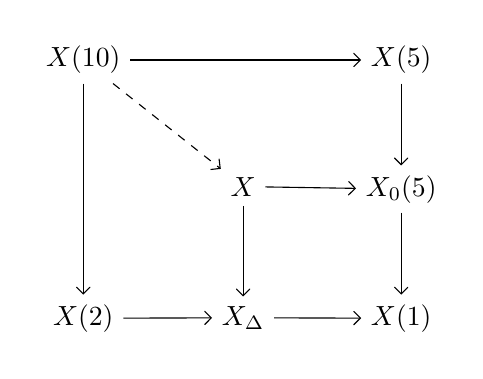
\begin{tikzpicture}[scale=2]
\matrix (m) [matrix of math nodes, row sep=3em, column sep=3em]
{ X(10) & & X(5)  \\
 & X & X_0(5)  \\
X(2) & X_{\Delta} & X(1)\\};
\path[->,font=\scriptsize,>=angle 90]
(m-1-1) edge  (m-3-1)
(m-1-1) edge (m-1-3)
(m-1-3) edge  (m-2-3)
(m-1-1) edge[dashed]  (m-2-2)
(m-2-3) edge  (m-3-3)
(m-2-2) edge  (m-2-3)
(m-2-2) edge  (m-3-2)
(m-3-1) edge  (m-3-2)
(m-3-2) edge  (m-3-3);
\end{tikzpicture}
\end{center}
where $X$ is the normalization of the fiber product $X_{\Delta} \times_{X(1)} X_0(5)$.  $X$ is an elliptic curve given by the equation
\[X: \qquad  y^2 = x^3 + 22x^2 +125x .\]
The map to $X_{\Delta}$ is given by
\[ (x,y) \mapsto \frac{y(x^2-500x -15625)}{x^3}. \]
Sage easily determines that $X$ is rank $0$, with rational points $(0:0:1)$ and $(0:1:0)$, both lying in the kernel of the map to $X_{\Delta}$.  Thus our elliptic curve cannot give rise to a rational point on $X_0(5)$, and we conclude that $\rho_{E,5}$ is irreducible and thus absolutely irreducible.
\end{proof}



\vspace{100pt}

\section{The Frey-Mazur Conjecture and Theorem 1.2}


\section{Examples}



















\bibliography{bib}{}
\bibliographystyle{amsalpha}


\end{document}